\documentclass{article}

% if you need to pass options to natbib, use, e.g.:
%     \PassOptionsToPackage{numbers, compress}{natbib}
% before loading neurips_2019

% ready for submission
% \usepackage{neurips_2019}

% to compile a preprint version, e.g., for submission to arXiv, add add the
% [preprint] option:
    % \usepackage[preprint]{neurips_2019}

% to compile a camera-ready version, add the [final] option, e.g.:
\usepackage[final]{neurips}

% to avoid loading the natbib package, add option nonatbib:
    % \usepackage[nonatbib]{neurips_2019}
\usepackage{multicol}
\usepackage{float}
\usepackage[center]{caption}

\usepackage[utf8]{inputenc} % allow utf-8 input
\usepackage[T1]{fontenc}    % use 8-bit T1 fonts
\usepackage{hyperref}       % hyperlinks
\usepackage{url}            % simple URL typesetting
\usepackage{booktabs}       % professional-quality tables
\usepackage{amsfonts}       % blackboard math symbols
\usepackage{nicefrac}       % compact symbols for 1/2, etc.
\usepackage{microtype}      % microtypography
\usepackage{graphicx}
\usepackage{amsmath}
\usepackage{xepersian}

\settextfont{XB Yas.ttf}

\title{
پروژه‌ی پایانی\\
تبدیل مسئله‌ی انتخاب ویژگی یا
\lr{Feature selection}
به یک مسئله‌ی بهینه‌سازی و ارائه‌ی روش حل توسط الگوریتم فراابتکاری شبیه‌سازی تبرید یا
\lr{Simulated annealing}
}


% The \author macro works with any number of authors. There are two commands
% used to separate the names and addresses of multiple authors: \And and \AND.
%
% Using \And between authors leaves it to LaTeX to determine where to break the
% lines. Using \AND forces a line break at that point. So, if LaTeX puts 3 of 4
% authors names on the first line, and the last on the second line, try using
% \AND instead of \And before the third author name.

\author{%
    گروه \lr{B}\\
  امیرحسین مهدی‌نژاد\\
  شماره دانشجویی 810800058\\
  \texttt{mahdinejad@ut.ac.ir} \\
  % examples of more authors
  % \And
  % Coauthor \\
  % Affiliation \\
  % \texttt{email} \\
  % \AND
  % Coauthor \\
  % Affiliation \\
  % Address \\
  % \texttt{email} \\
}

% create title (includes both anonymized and non-anonymized versions)
% \providecommand{\@makepertitle}{}
% \newcommand{\makepertitle}{%
%   \vbox{%
%     \hsize\textwidth
%     \linewidth\hsize
%     \vskip 0.1in
%     \toptitlebar
%     \centering
%     {\LARGE\bf \@title\par}
%     \bottomtitlebar
%       \def\And{%
%         \end{tabular}\hfil\linebreak[0]\hfil%
%         \begin{tabular}[t]{c}\bf\rule{\z@}{24\p@}\ignorespaces%
%       }
%       \def\AND{%
%         \end{tabular}\hfil\linebreak[4]\hfil%
%         \begin{tabular}[t]{c}\bf\rule{\z@}{24\p@}\ignorespaces%
%       }
%       \begin{tabular}[t]{c}\bf\rule{\z@}{24\p@}\@author\end{tabular}%
%     \vskip 0.3in \@minus 0.1in
%   }
% }

\begin{document}


\begin{minipage}{0.1\textwidth}% adapt widths of minipages to your needs

\includegraphics[width=1.1cm]{Photos/UT_logo.png}
\end{minipage}%
\hfill%
\begin{minipage}{0.9\textwidth}\raggedleft
دانشکده فنی، دانشگاه تهران\\
الگوریتم‌های گراف و شبکه - 
بهمن
ماه 1400\\
\end{minipage}
% \end{}


\makepertitle


% \begin{abstract}
%  این بخش از یک پاراگراف تشکیل شده است که توضیحاتی کلی در مورد مساله و راه حل شما ارائه می‌دهد.
% \end{abstract}

\begin{multicols}{2}
\section{
مقدمه
}
هدف از حل مسئله‌ی انتخاب ویژگی، انتخاب یک زیرمجموعه از بین ویژگی‌ها یا متغیرهایی است که آن‌ها را متغیرهای مستقل فرض می‌کنیم که طی فرآیندی متغیر وابسته را ایجاد می‌کنند.\\
لزوما استفاده از تمام
{n}
ویژگی به نفع ما نیست و به همین خاطر به انتخاب زیرمجموعه‌ای از ویژگی‌ها می‌پردازیم. 
راه حل قطعی برای این مسئله وجود ندارد، در نتیجه به روش‌های دیگری همچون استفاده از الگوریتم‌های فراابتکاری روی می‌آوریم.\\
ما ویژگی‌ها را همانطور که هستند انتخاب می‌کنیم و با مسئله‌ای باینتری مواجه هستیم.
بدین منظور ویژگی‌های انتخاب شده را وارد یکی از مدل‌های یادگیری ماشین نظارت شده می‌کنیم و هرچه اختلاف خروجی این مدل با اختلاف خروجی هدف کمتر باشد، به مجموعه جواب بهتری رسیده‌ایم و می‌خواهیم این اختلاف را کمینه کنیم.
$$y = f(x) \simeq \hat{f}(\hat{x})$$
$$\hat{x} \subseteq x$$

\section{
الگوریتم شبیه‌سازی تبرید
}
برای حل این مسئله از الگوریتم شبیه‌سازی تبرید یا
\lr{Simulated annealing}
استفاده می‌کنیم که در آن از فرآیند بازپخت که از مباحث رشته‌ی متالوژی محسوب می‌شود، الگو گرفته شده است.\\
در واقع ابتدا جواب‌های مسئله با نوسانات زیادی تغییر می‌کنند (
\lr{Exploration}
) و سپس به تدریج دامنه‌ی تغییرات کم می‌شود و به سمت جواب بهینه هدایت می‌شویم.\\
این الگوریتم از یک نقطه‌ی دلخواه آغاز به کار کرده و سپس یک حالت همسایه را انتخاب می‌کند. پس از آن به طور احتمالی تصمیم می‌گیرد که در حالت کنونی بماند یا به حالت همسایه‌ای جابجا شود. این کار تا جایی انجام می‌شود که سیستم به یک حالت عقلانی برسد یا اینکه میزان محاسبات، از یک آستانه‌ی مشخص بیشتر شود.\\
برای فرار از گیر کردن در بهینه‌ی محلی از این ایده استفاده می‌شود که مانع از انجام حرکت‌های بد نشویم (یعنی امکان حرکت به سمت همسایه‌های کم‌ارزش‌تر وجود داشته باشد) و سپس به تدریج اندازه و تعداد حرکت‌های بد را کاهش دهیم.\\
با در نظر گرفتن متغیر
\lr{T}
به عنوان دما، در هر مرحله از اجرای الگوریتم، حالت بعدی به صورت تصادفی انتخاب می‌شود. اگر حالت بعدی انتخاب شده از حالت فعلی بهتر باشد، به آن حالت می‌رویم و در غیر این صورت، با احتمال 
$e^{\Delta E/T}$
به آن حالت خواهیم رفت. یعنی هرچه حالت بعدی بدتر باشد، این احتمال به صورت نمایی کاهش یافته و همچنین با کاهش
\lr{T}
این احتمال کاهش می‌یابد.\\
هرچه دما آهسته‌تر کاهش یابد، تعداد مراحل جستجو و در نتیجه احتمال یافتن بهینه‌ی سراسری بیشتر است.

\section{
نحوه‌ی مدل‌سازی
}
دیتاستی که در اختیار ما قرار گرفته است شامل ۱۱ ویژگی برای پیش‌بینی نارسایی قلبی است. پس جوابی که با آن الگوریتم شبیه‌سازی تبرید را شروع می‌کنیم، آرایه‌ای ۱۱ عنصری از صفر و یک‌هاست
(انتخاب یا عدم انتخاب یک ویژگی برای آموزش).\\
در هر مرحله از اجرای الگوریتم با توجه به توضیحاتی که در بخش قبلی به آن اشاره شد، با یک روش یادگیری نظارت‌شده مثل
\lr{SVM}
که برای مسائل طبقه‌بندی استفاده می‌شود، جواب بدست آمده را با ستون ۱۲ام مقایسه می‌کنیم و آن را به عنوان معیار امتیازدهی در نظر می‌گیریم.\\
در مورد الگوریتم 
\lr{SA}
گفته می‌شود که اگر دما به آرامی کاهش یابد، الگوریتم پاسخ بهینه سراسری را با احتمالی که به سمت یک میل می‌کند، پیدا خواهد نمود.

\section{
پیاده‌سازی
}
پروژه متشکل از سه فایل است:
\begin{itemize}
    \item \lr{SA.py}\\
    الگوریتم
    \lr{Simulated Annealing}
    به صورت یک تابع در این فایل پیاده‌سازی شده است تا در فایل‌های دیگر مورد استفاده قرار گیرد.
    \item \lr{FS.py}\\
    دسته‌بندی با استفاده از
    \lr{SVM}
    در این فایل به صورت یک تابع
    \lr{evaluate}
    پیاده‌سازی شده است و هریک از جواب‌های تولید شده را با توجه به
    \lr{score}
    آن ارزیابی می‌کنیم.
    \item \lr{testing.ipynb}\\
    محیطی برای تست کردن نتیجه‌ی الگوریتم و همچنین اجرای الگوریتم یادگیری بر روی تمام ویژگی‌هاست.
\end{itemize}
به تفصیل به شرح هرکدام از این فایل‌ها خواهیم پرداخت.

\subsection{
پیاده‌سازی الگوریتم فراابتکاری
}
همان‌طور که اشاره شد در فایل
\lr{SA.py}
این الگوریتم به صورت یک تابع پیاده شده است. در بخش ۳ گفتیم که ویژگی‌های ما به صورت آرایه‌ای ۱۱ عنصری از بیت‌های صفر یا یک هستند؛ پس هرکدام از جواب‌ها یک آرایه به همین شکل هستند و در نهایت قرار است بهترین آرایه از صفر و یک‌ها را ارائه کنیم که همان جواب نهایی ماست.

\subsubsection{
تابع
\lr{generate\_candidate}
}
همسایه‌ها را برای ما تولید می‌کند. متغیر
\lr{distance}
که مقدار پیش‌فرض آن یک است در واقع فاصله‌ی ما با همسایه را مشخص می‌کند. یعنی خانه‌ی همسایه یک بیت با آرایه‌ی جواب فعلی متفاوت است که البته می‌توان آن را بر حسب
\lr{T}
نیز مشخص کرد ولی تاثیر چندانی بر الگوریتم ندارد.\\
اندیس‌هایی که قرار است متفاوت شوند (که در اینجا فقط یک اندیس است) تولید شده و
\lr{NOT}
می‌شود.
\begin{figure}[H]
    \centering
    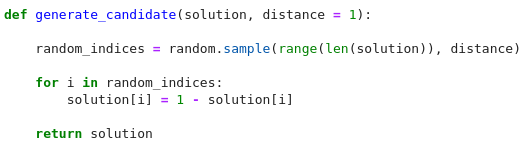
\includegraphics[width=0.99\linewidth]{Photos/SA/gencandid.png}
    \caption{
    \lr{generate\_candidate}
    }
    \label{fig:my_label}
\end{figure}

\subsubsection{
تابع
\lr{binary\_simulated\_annealing}
}
همان تابع اصلی ماست. طول ویژگی‌ها یا
\lr{features\_len}
اینجا به صورت پیشفرض ۱۱، تعداد اجراها یا
\lr{n\_iterations}
برابر با ۱۰۰۰ و دمای اولیه یا
\lr{temperature}
برابر با ۵۰ در نظر گرفته شده است.

ابتدا جوابی به صورت رندوم تولید شده و با استفاده از فایل
\lr{FS.py}
تابع امتیازدهی یا همان
\lr{evaluate}
انجام شده است. جواب فعلی و امتیاز فعلی همان بهترین جواب و بهترین امتیاز هستند که به عنوان حالت اولیه چاپ می‌شوند.
\begin{figure}[H]
    \centering
    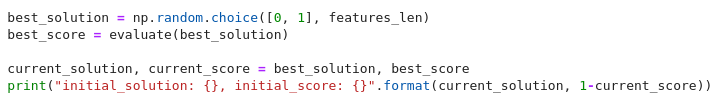
\includegraphics[width=0.99\linewidth]{Photos/SA/randsol.png}
    \caption{
    \lr{random\_solution}
    }
    \label{fig:my_label}
\end{figure}

به تعداد
\lr{n\_iterations}
هر دفعه یک همسایه تولید شده و امتیاز آن همسایه نیز با توجه به همان تابع
\lr{evaluate}
بدست می‌آید و در صورتی که خطا کمتر از خطایی بود که تا الآن داشتیم، بهترین جواب و بهترین امتیازی که داشیم را آپدیت کرده و این گام از الگوریتم را چاپ می‌کنیم.
\begin{figure}[H]
    \centering
    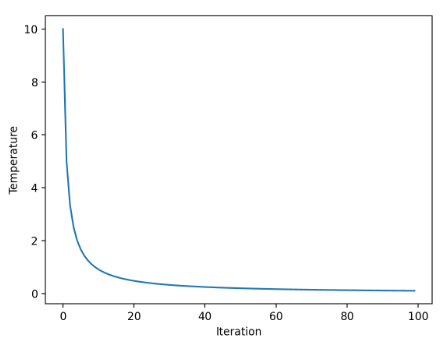
\includegraphics[width=0.99\linewidth]{Photos/SA/temperature.png}
    \caption{
    نمودار کم شدن دما بر حسب دفعات اجرا
    }
    \label{fig:my_label}
\end{figure}

در اینجا
$\Delta E$
همان متغیر
\lr{delta}
ی ماست که اختلاف
\lr{score}
ها را در آن نگه داشتیم و 
\lr{T}
فعلی دما تقسیم بر مرحله‌ای است که در آن هستیم. هرچقدر که جلوتر می‌رویم این مقدار کمتر می‌شود و به علت جلوگیری از تقسیم بر صفر، تقسیم بر
\lr{i+1}
شده است. یعنی دما به صورت نمایی کمتر می‌شود و احتمال همان
$e^{\Delta E/T}$
است که عدد رندومی تولید شده و با آن مقایسه می‌شود که اگر کمتر بود جابجایی اتفاق بیوفتد.
\begin{figure}[H]
    \centering
    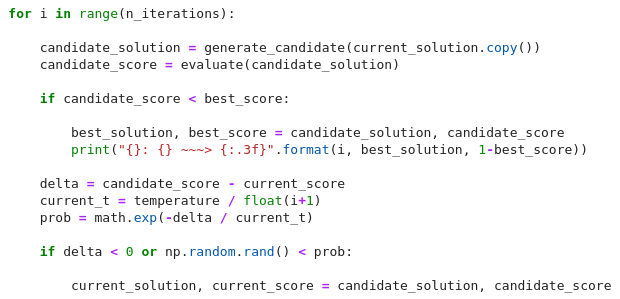
\includegraphics[width=0.99\linewidth]{Photos/SA/algorithm.png}
    \caption{
    بدنه‌ی تکرار الگوریتم
    }
    \label{fig:my_label}
\end{figure}

در نهایت بهترین جواب و بهترین امتیاز را
\lr{return}
می‌کنیم که بعدا از آن استفاده شود.

\subsection{
پیاده‌سازی کلاس‌بندی با استفاده از تمام ویژگی‌ها
}
در فایل
\lr{testing.py}
ابتدا
\lr{dataframe}
را خوانده و چند ردیف اول آن را مشاهده می‌کنیم.\\
از کتابخوانه‌ی
\lr{sklearn}
و از بخش
\lr{preprocessing}
به سراغ
\lr{LabelEncoder}
می‌رویم تا دیتاهای
\lr{categorical}
یا در واقع مقادیری که عددی نیستند را به صورت عدد برچسب‌گذاری کرده و جایگزین آن‌ها کنیم.
\begin{figure}[H]
    \centering
    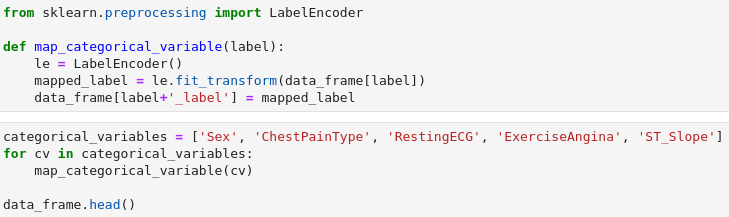
\includegraphics[width=0.99\linewidth]{Photos/SA/label_encoder.png}
    \caption{
    \lr{label\_encoder}
    }
    \label{fig:my_label}
\end{figure}

تابع
\lr{map\_categorical\_variable}
به همین منظور تعریف شده است که برچسب‌ها را دریافت کرده و به مقادیر عددی مپ کند. برای تک‌تک این مقادیر گسسته، تابع صدا زده شده و برچسب عددی تولید شده به صورت ستون‌هایی به
\lr{dataframe}
اضافه می‌شوند و در نهایت خود آن مقادیر را
\lr{drop}
می‌کنیم چون نیازی به آن‌ها نیست. الآن همه‌ی داده‌های ما مقادیر عددی هستند.

نمودار تقابل
\lr{feature}
ها به صورت جدولی ۱۱ در ۱۱ رسم شده‌است که در آن یک بودن
\lr{HeartDisease}
با رنگ قرمز و صفر بودن آن با رنگ آبی مشخص شده است. با استفاده از این نمودارها و همچنین خروجی
\lr{describe}
می‌توان دید خوبی نسبت به داده‌ها پیدا کرد.
\begin{figure}[H]
    \centering
    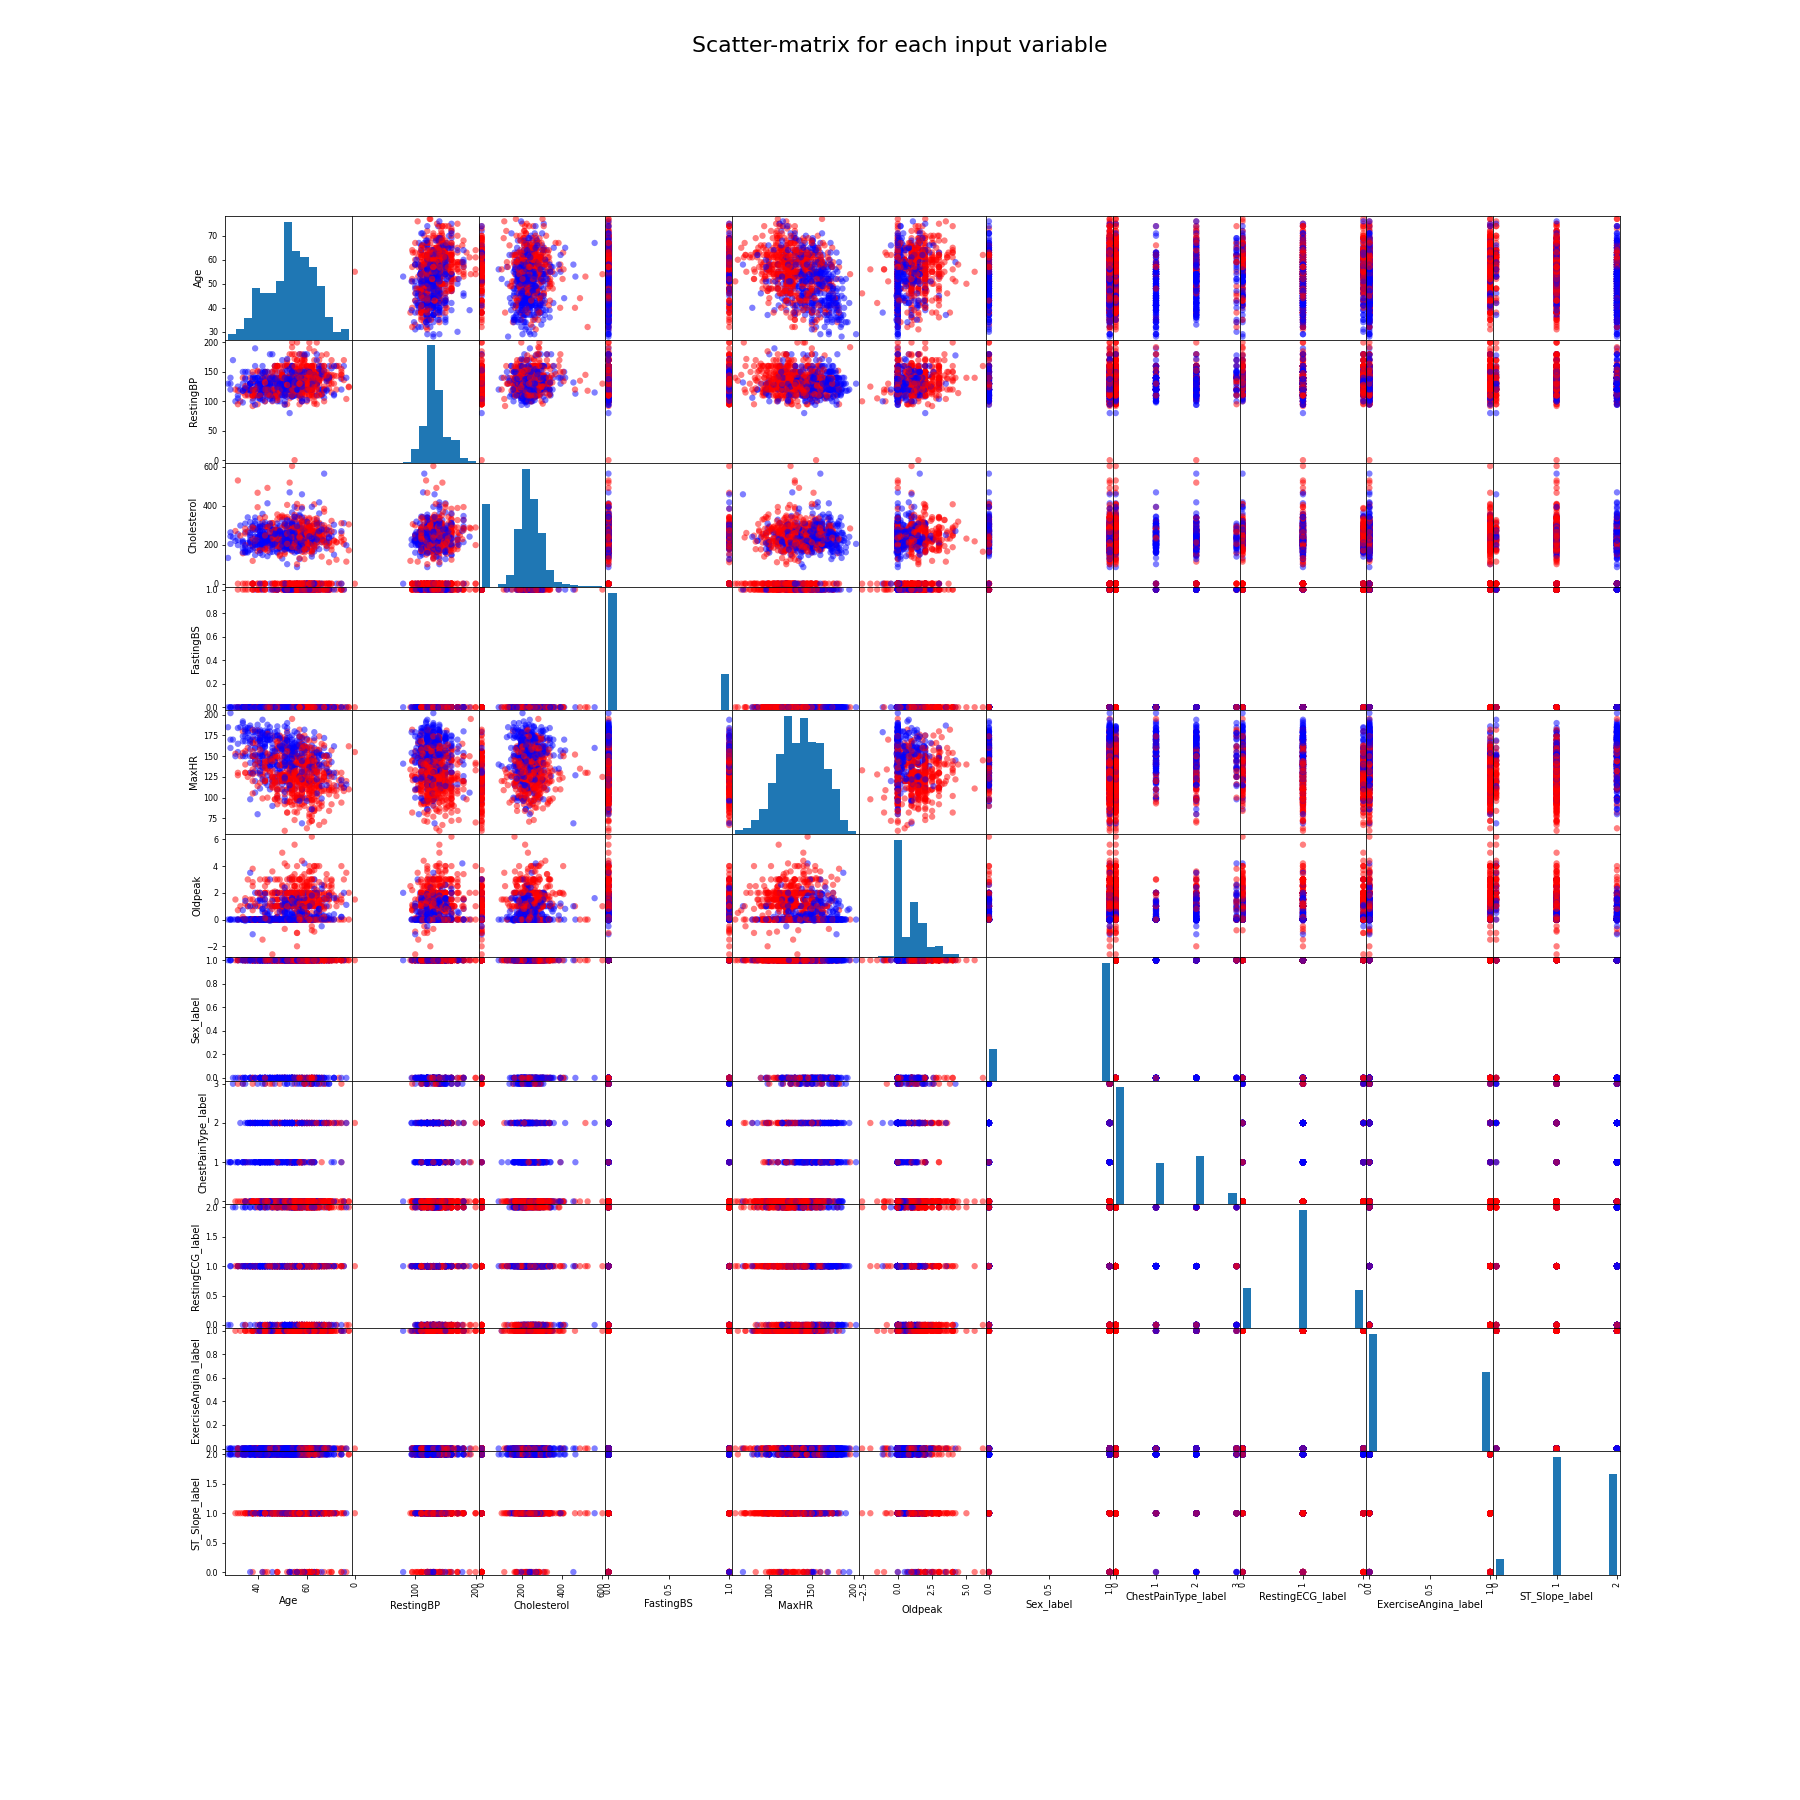
\includegraphics[width=0.99\linewidth]{Photos/SA/scatter_matrix.png}
    \caption{
    \lr{scatter\_matrix}
    }
    \label{fig:my_label}
\end{figure}

با کمک
\lr{train\_test\_split}
از کتابخوانه‌ی
\lr{sklearn.model\_selection}
داده‌ها را به نسبت ۳۰ - ۷۰ بین تست و تمرین توزیع می‌کنیم. همچنین با بکارگیری
\lr{MinMaxScaler}
مقیاس داده‌ها را نرمال می‌کنیم تا آن‌ها برای استفاده در
\lr{classifier}
ها آماده شوند.\\
همان‌طور که قبل‌تر اشاره شده بود ما از
\lr{SVM}
برای کلاس‌بندی استفاده کردیم. داده‌ها 
\lr{fit}
شده و دقت یا 
\lr{score}
در نهایت با در نظر گفتن همه‌ی ویژگی‌ها تقریبا ۸۷ درصد برای داده‌های تمرین و ۸۸ درصد برای داده‌های تست بدست آمد.
\begin{figure}[H]
    \centering
    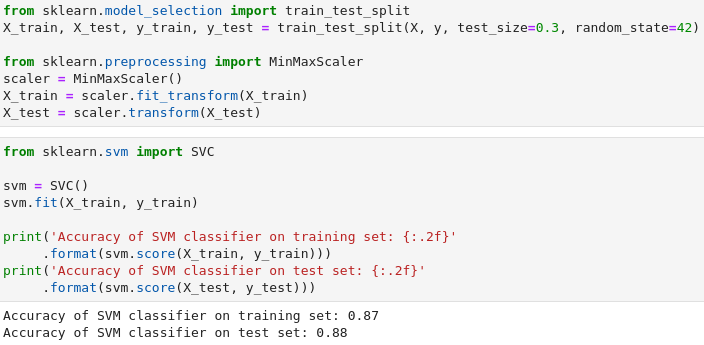
\includegraphics[width=0.99\linewidth]{Photos/SA/learning.png}
    \caption{
    کلاس‌بندی با تمام فیچرها
    }
    \label{fig:my_label}
\end{figure}

با اضافه کردن 
\lr{binary\_simulated\_annealing}
از فایل
\lr{SA.py}
با همان مقادیر گفته شده در بخش‌های قبلی، امتیازات بدست آمده از جواب‌ها در همین پروسه‌ی کلاس‌بندی گفته شده، به صورت تابع درآمده و با یکدیگر مقایسه شد. در بخش بعدی به توضیحات همین تابع می‌پردازیم.

\subsection{
تابع ارزیابی و انتخاب ویژگی
}
در فایل
\lr{FS.py}
تابع ارزیابی، دقیقا معادل با همان کدهایی که در فایل
\lr{testing.ipynb}
پیاده شده بود، ولی ضمن در نظر گرفتن آرایه‌ی باینری
\lr{solution}
که خروجی الگوریتم
\lr{SA}
است، مورد استفاده قرار گرفت.
\begin{figure}[H]
    \centering
    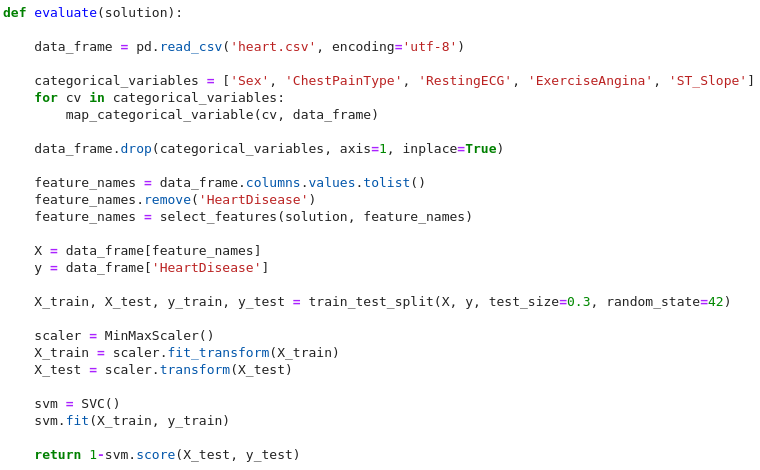
\includegraphics[width=0.99\linewidth]{Photos/SA/evaluate.png}
    \caption{
    \lr{evaluate}
    }
    \label{fig:my_label}
\end{figure}

\subsubsection{
تابع
\lr{select\_features}
}
آرایه‌ی
\lr{solution}
دریافت شده را گرفته و ویژگی‌هایی که انتخاب شده‌اند (معادل با خانه‌هایی از آرایه که یک هستند) را به عنوان پاسخ برمی‌گرداند.
\begin{figure}[H]
    \centering
    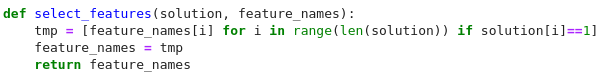
\includegraphics[width=0.99\linewidth]{Photos/SA/select_features.png}
    \caption{
    \lr{select\_features}
    }
    \label{fig:my_label}
\end{figure}

هر سری تمام این عملیات در تابع ارزیابی تکرار می‌شود و طبق توضیحاتی که در بخش قبلی به آن‌ها اشاره شد، آموزش انجام می‌گیرد. در واقع دسته‌بندی مشابه همان چیزی که در فایل
\lr{testing.ipynb}
دیدیم، اینجا نیز انجام می‌شود و مقدار
\lr{score}
در نهایت به عنوان امتیاز این جواب برگردانده می‌شود.

\begin{figure}[H]
    \centering
    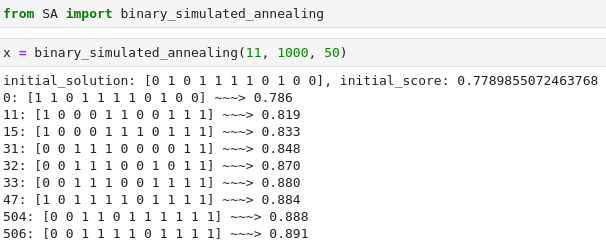
\includegraphics[width=0.99\linewidth]{Photos/SA/finalresult.png}
    \caption{
    نتیجه‌ی نهایی
    }
    \label{fig:my_label}
\end{figure}
با انتخاب نکردن ۳ تا از ویژگی‌ها در اجرای ۵۰۶ام به بهترین جواب رسیدیم که دقت آن حدود یک درصد از حالتی که تمام فیچرها را در نظر گرفته بودیم (قطعه کدی که در فایل
\lr{testing.ipynb}
بررسی شد) بهتر عمل کرد.

\begin{figure}[H]
    \centering
    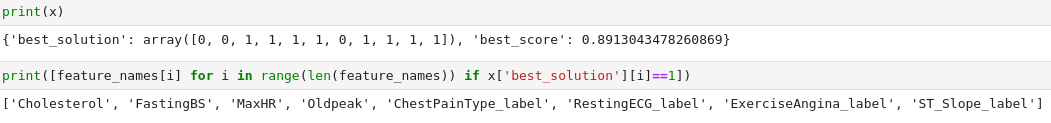
\includegraphics[width=0.99\linewidth]{Photos/SA/featuresfinal.png}
    \caption{
    ویژگی‌هایی که انتخاب شدند
    }
    \label{fig:my_label}
\end{figure}

\section{
منابع
}
\lr{1. Agrawal P, Abutarboush HF, Ganesh T, Mohamed AW. Metaheuristic Algorithms on Feature Selection: A Survey of One Decade of Research (2009-2019). IEEE Access [Internet]. Institute of Electrical and Electronics Engineers (IEEE); 2021;9:26766–91.}\\
\lr{2. Lin S-W, Lee Z-J, Chen S-C, Tseng T-Y. Parameter determination of support vector machine and feature selection using simulated annealing approach. Applied Soft Computing [Internet]. Elsevier BV; 2008 Sep;8(4):1505–12.}

\end{multicols}
\end{document}
